%!TEX root = ../main.tex
\section{The CoALA Framework}
\ac{CoALA} positions the \ac{LLM} as the core component of a larger cognitive
architecture, where a language agent stores information in \textbf{memory}
modules, and acts in an action space structured into external and internal
parts, as shown in \Cref{fig:coala}.
%
\begin{figure}[ht]
    \centering
    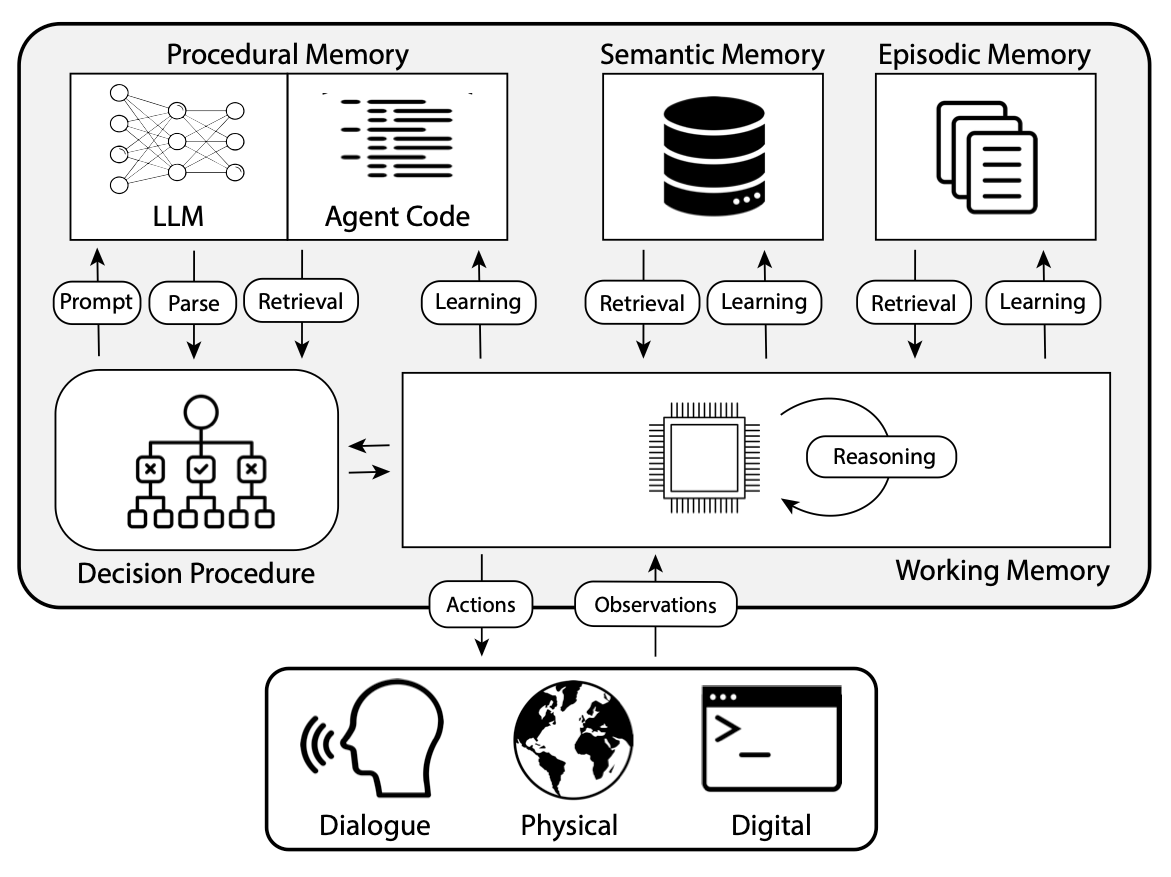
\includegraphics[width=0.4\textwidth]{img/coala-architecture.png}
    \caption{The \ac{CoALA} architecture, defining a set of interacting modules
    and processes.}
    \label{fig:coala}
\end{figure}
%
External actions let the agent interact with external environment through
\emph{grounding}, while internal actions consist of a set of interactions with
internal memories, and can be decomposed into
\begin{enumerate*}[label=(\emph{\roman{*}})]
    \item \emph{retrieval} when reading from long term memory,
    \item \emph{reasoning} with updates of the short term working memory with
        the \ac{LLM} and
    \item \emph{learning} by means of writing in long term memory.
\end{enumerate*}

\ac{CoALA} leverages key concepts inspired by decades of research in cognitive
agents, yet the incorporation of an \ac{LLM} lead to the addition of
\emph{reasoning actions}, which can \textbf{flexibly produce new knowledge} for
various purposes.

\subsection{Memory}
Memory is necessary due to the \emph{stateless} nature of \ac{LLM}s, which has
been already shown by language agents to improve drastically agent's and
accuracy. Under the \ac{CoALA} framework agents organise information into
multiple memory modules, which we'll describe in the following paragraphs.

\paragraph{Working Memory} maintains active and readily available information
for the \emph {current decision cycle}, including perceptual input, active
reasoning and other information carried by the previous decision cycle. In
short, the working memory synthesise \ac{LLM}s input from a subset of working
memory, and its output is then parsed back into other variables which are
stored back in working memory and used to execute the corresponding action.
Finally, the working memory also interact with long-term memories and
grounding.

\paragraph{Episodic Memory} stores experiences from earlier decision cycles
which can be encoded in various formats. This memory can then be accessed by
the working memory during the \emph{planning stage} of a decision cycle to
support \emph{reasoning}.

\paragraph{Semantic Memory} stores an agent's \emph{knowledge} about the
\emph{world} and \emph{itself}. In language agents this memory is not
fixed/read-only but agents can write new knowledge obtained from \ac{LLM}
reasoning as a form of learning (incrementally build up knowledge from
experience).

\paragraph{Procedural Memory} divided in two forms

\begin{itemize}
    \item \emph{implicit} knowledge stored in the \ac{LLM} weights;
    \item \textbf{explicit} knowledge written in the agent's code, furthermore
        divisible into \emph{procedures} which implement \emph{actions} (reasoning,
        retrieval grounding and learning), and \emph{procedures} that implement \emph{decision-making} itself.
\end{itemize}

Unlike other memories, procedural memory \textbf{must be initialised} by the
designer, and finally, even if possible, learning by writing new actions into
this memory is \emph{riskier} as it can easily introduce bugs or allow an
agents to subvert its designer's intentions.

\subsection{Grounding Actions}
Grounding procedures execute internal actions and \emph{process environmental
feedback} into working memory as text.

\paragraph{Physical Environment} it involves processing inputs into textual
observations, and affect the physical environments via robotic planners that
take \emph{language-based commands}. When it comes to perceptual inputs,
\textbf{vision-language models} are typically used to convert images into
text~\cite{alayrac2022flamingovisuallanguagemodel}, providing additional
context for the \ac{LLM}.

\paragraph{Dialogue with Humans or Other Agents} by means of classical
linguistic interaction can let the agent to accept new instructions or learn
from people, and for agents capable of generating language they can ask for
clarification, collaborate with multiple agents for social simulations or
collaborative task solving.

\paragraph{Digital Environment} including interactions with games, APIs, as well as
\emph{general code execution}, resulting in cheaper, faster and thus a more convenient
testbed for language agents.

\subsection{Retrieval Actions (Planning)}
Retrieval can be seen as a general procedure for reading information from long
term memories into working memory. We distinguish among various type of
retrieval:
\begin{itemize}
    \item \emph{Rule Based retrieval} useful for explicit memory organisation
        (e.g. designer's rules), providing deterministic result with limited
        flexibility and struggling with complex queries/fuzzy matches.
    \item \emph{Sparse Retrieval} relies on discrete representations, such as
        keywords or reverse indices. It is great for fast retrieval of factual
        information or structured knowledge, but struggles with \emph{semantic
        matching}.
    \item \emph{Dense Retrieval} is particularly useful for retrieving
        semantically relevant concepts. It uses continuous vector
        representations (\emph{embeddings}) and retrieves memories based on
        semantic similarities (e.g. nearest neighbours in a $d$-dimensional
        feature space), like
        BERT~\cite{devlin2019bertpretrainingdeepbidirectional} which uses a
        transformer-based embedding model.
\end{itemize}

\subsection{Reasoning Actions (Planning)}
Reasoning consists of a set of actions that aim to the processing of the
context of working memory to generate new information. With reasoning a
summarisation and distillation of core information inside working memory is
performed, gaining insights about most recent observations, most recent
trajectory and, optionally, information retrieved from long term memories.

Reasoning supports \emph{learning} by writing results in long term memory, and
\emph{decision making} by using the results as additional context for
subsequent \ac{LLM} calls.

\subsection{Learning}\label{ssec:learning}
Learning is essentially a writing process on long term memories, which includes
various kind of procedures explored in the following sections. This various
ways of learning allow language agents (e.g. with respect to \ac{RL} agents) to
learn rapidly by storing task-relevant language (quicker than parameter updates
for \ac{RL} agents).

\subsubsection{Updating Episodic Memory with Experience}
Following \ac{RL} common practice, store episodic trajectories to update a
\emph{parametric policy}. The experiences in this memory could be retrieved
later as examples and bases for reasoning and decision-making.

\subsubsection{Updating Semantic Memory with Knowledge}
Make use of \ac{LLM}s to reason about \emph{raw experiences} and store
resulting \emph{inference} in semantic memory (e.g. there's no dishwasher in
the room).

\subsubsection{Updating LLMs Parameters (Procedural Memory)}
Recall that \ac{LLM} weights represent a \textbf{implicit procedural
knowledge}. Weights can then be adjusted to an agent's domain by \emph{fine
tuning} during its lifetime, and this can be accomplished by supervised
learning, imitation learning, from environmental feedback or AI feedback,
typically using a measure of \emph{consistency} to select generations to fine
tune on~\cite{wang2023selfconsistencyimproveschainthought}. Fine tuning is a
costly form of Learning, but as training is becoming more efficient and some
optimised \ac{LLM}s techniques are being exploited, it may be possible to allow
language agent to autonomously determine when and how to fine-tune their
\ac{LLM}.

\subsubsection{Updating Agent's Code (Procedural Memory)}
\ac{CoALA} allows agents to update their source code; more in particular:
\begin{itemize}
    \item \textbf{Update reasoning} for example, infer prompt instructions
        (template) from input-output
        examples~\cite{zhou2023largelanguagemodelshumanlevel};
    \item \textbf{Update grounding actions}: notably current methods are limited
        to creating new code skills to interact with external environment.
    \item \textbf{Update retrieval}, not yet studied because it is considered a
        basic action designed with some fixed implementation; however \ac{LLM}s
        can perform distillation or use other techniques to learn \emph{better
        retrieval processes}.
    \item \textbf{Update learning} or \textbf{decision making} is theoretically
        possible, however risky for the agent's functionality and alignment.
\end{itemize}

\subsection{Decision Making}
\begin{figure}[ht]
    \centering
    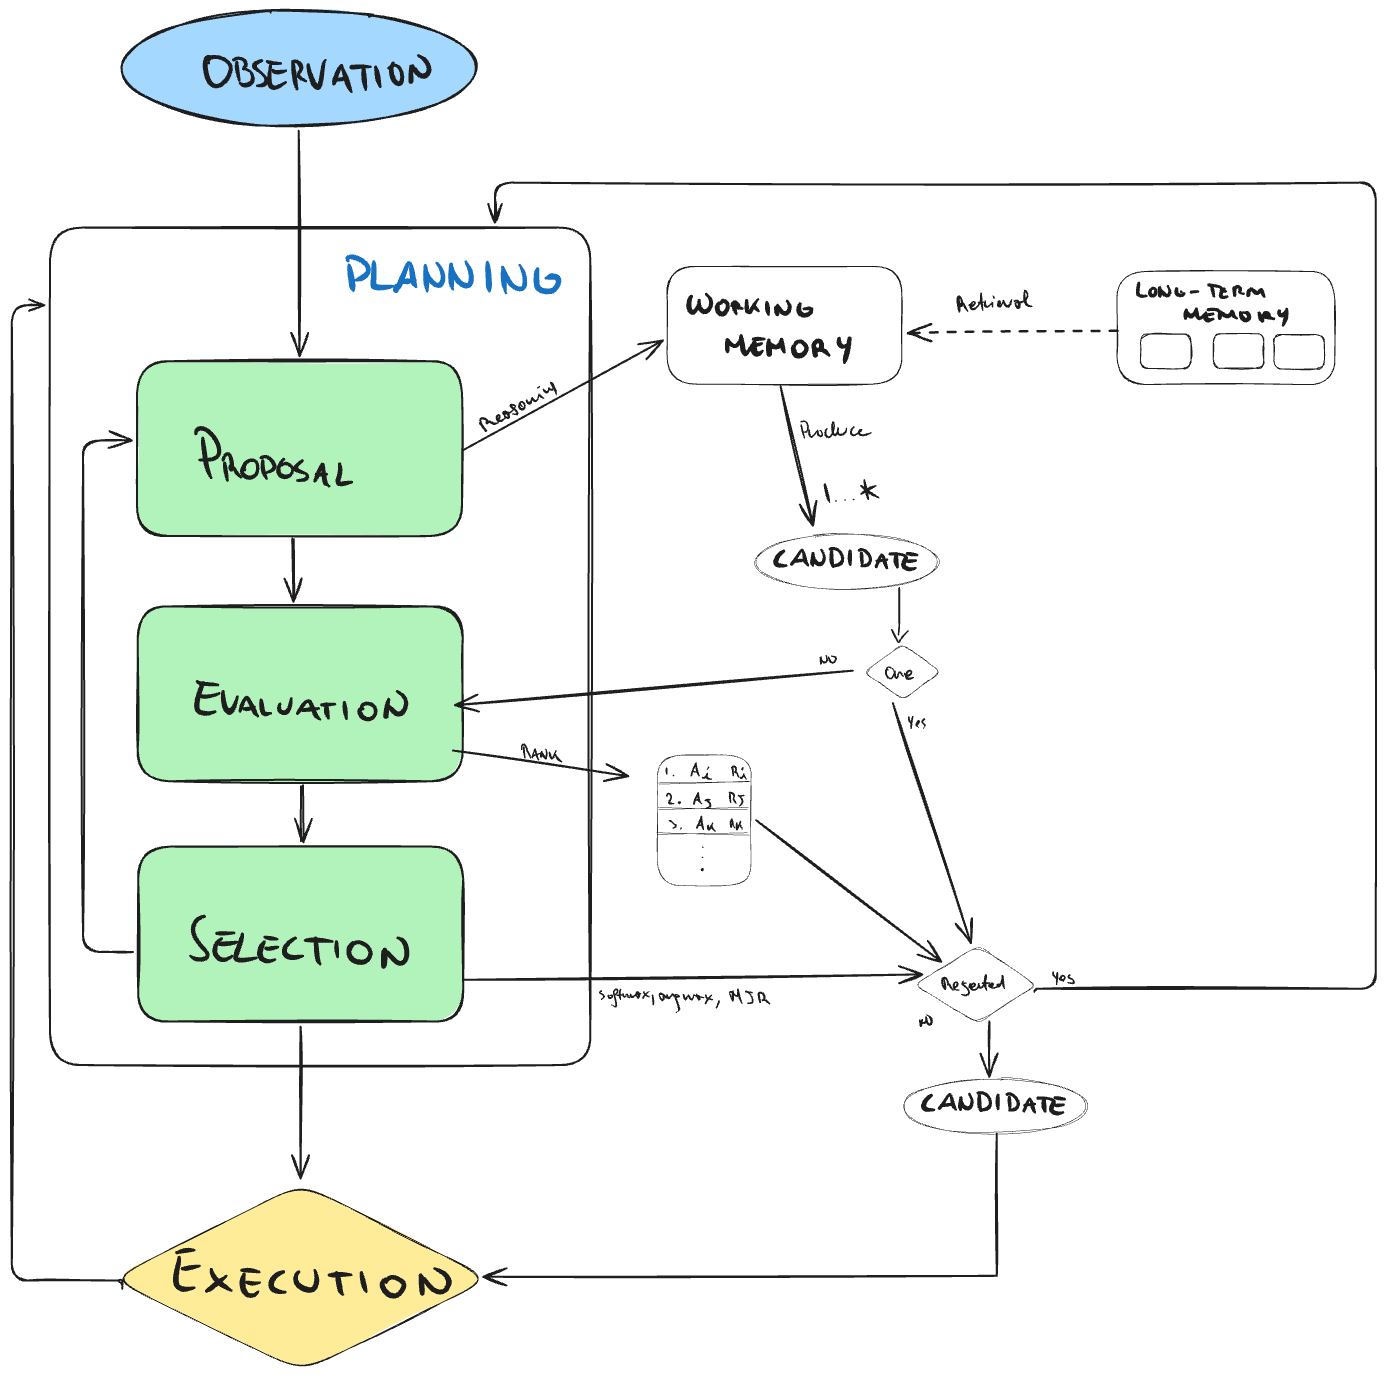
\includegraphics[width=0.4\textwidth]{img/coala-decision-making.pdf}
    \caption{The \ac{CoALA} decision making process, highlighting its building
        blocks (left) with the way they interact and interleave during the actual
        loop, by means of the decision tree (right).}
    \label{fig:coala-decision-making}
\end{figure}
Decision making is the procedure that chooses which action to apply, structured
into decision cycles which yield an external grounding action or internal
learning action.
In \Cref{fig:coala-decision-making} is shown the decision loop, integrated as well
with a simple custom decision tree. We can then summarise briefly its components:
\begin{itemize}
    \item \textbf{Planning Stage} where reasoning and retrieval can be applied
        to propose, evaluate and select actions. These sub-stages can iterate
        to build \emph{mulit-step} simulations before taking an action,
        improving at each cycle the candidate solution. Each cycle includes:
        \begin{enumerate}
            \item \emph{Proposal} where one or more action candidates are
                generated (using reasoning and optionally retrieval)a to sample
                one or more grounding actions from the \ac{LLM}.
            \item \emph{Evaluation} if multiple actions are proposed, for each
                one of them a value is assigned, either through heuristics,
                \ac{LLM} (perplexity) scores, or \ac{LLM} reasoning (useful for
                simulating grounding feedback from external
                world~\cite{hao2023reasoninglanguagemodelplanning})
            \item \emph{Selection} (through argmax, softmax or other like
                majority vote rule) of an action to execute, or reject them.
        \end{enumerate}
    \item \textbf{Execution}: selected action is applied executing relevant
        procedure from agent's source code. This can lead (depending on agent's
        implementation) to an external grounding action or an internal learning
        action.
\end{itemize}
%
After execution, an observation can be made from the environment, providing
feedback from the agent's action and the cycle loops again.
